\chapter{Read categorization}

Assuming that the majority of obtained SDKs are in fact discriminative, we can postulate a hypothesis : the more SDKs two reads share, the more likely they are to originate from the same haplotype.

Using the number of shared SDKs as a metric, we can restate our categorization problem as a graph problem. We can treat the reads as vertices and the number of shared SDKs between reads as weights of edges between the vertices. From here on out, we will be using the terms “read” and “vertex” interchangeably. We will refer to edges connecting reads or components of the same haplotype as "correct" and to those connecting different haplotype reads as "incorrect".


Our goal then is to identify components in the graph, such that their size is maximized, while also maximizing their “purity” - that is, keeping the proportion of reads from one haplotype in the component as high as possible.


We cannot expect to always find only two large components - that can only be done for a single chromosome diploid organism with high enough density of SDKs. The best we can hope for is finding $2N$ large components for a diploid organism with $N$ chromosomes. In case of our ENP75 and EPB75 datasets $N = 1$, since E.coli only has one chromosome.


We also do not hope to categorize all of the reads - inevitably, there will be many reads that are too short, contain too many errors, or do not carry enough information in their SDKs to be unambiguously categorized. However, as long as the reads in both determined categories span all the regions in the reference haplotype with sufficient coverage, eventual assembly of the reads should still yield high quality contigs.


Small inconsistency in categorized reads is also acceptable using the same reasoning. As long as we end up with significantly more reads of the correct origin covering the same region compared to the incorrect ones, we can expect the assembler to deal with such inconsistencies in the same way it deals with sequencing errors - by creating a consensus sequence.

\section{Spectral clustering}

Assuming that vertices connected by edges with strong weights should belong into the same component, we can approach the problem of creating said components through clustering.


While the sample graph on the left side of figure \ref{fig:spectral_example} is suggestively drawn in 2 dimensions with vertices already pre-arranged, the graphs we are really dealing with have no such form.


In order for ordinary clustering algorithms (such as K-means) to work, we first have to project our graph into a Euclidian space in such a way that the vertices we expect to be clustered together are separated only by a small distance, while those not clustered together are comparatively far apart.


One such way is spectral embedding\cite{luo2003spectral}. Suppose we have $N$ objects with a defined similarity metric. Given a $N \times N$ similarity matrix $A$, a spectrum of a graph is computed as eigenvalues and eigenvector of Laplacian of $A$. 
Spectral embedding enables us to use the columns of the first $d$ eigenvectors (when sorted by their respective eigenvalues) as coordinates in a $d$-dimensional coordinate space. 
Through this embedding, elements that have a high similarity as specified in $A$ are placed close (in terms of standard euclidian distance) together, while the dissimilar elements are further apart.

An example of such embedding into two dimensions can be seen on the right side of figure \ref{fig:spectral_example}.
As can be seen from a visualization, a graph embedded using this process is quite viable as an input to a run-of-the-mill clustering algorithm.

\begin{figure}
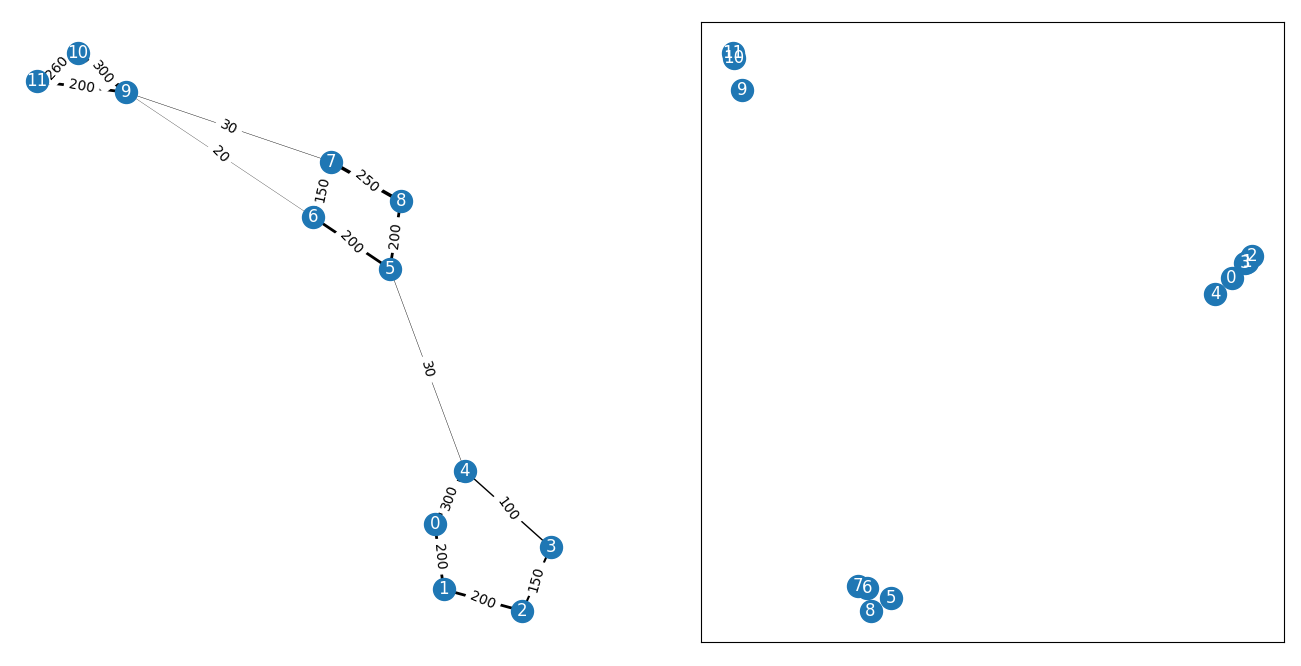
\includegraphics[width=400bp]{figures/spectral_example.png}

\caption{Example of spectral embedding. On left side force-directed layout, on right side embedding into 2D space}
\label{fig:spectral_example}
\end{figure}


\begin{figure}
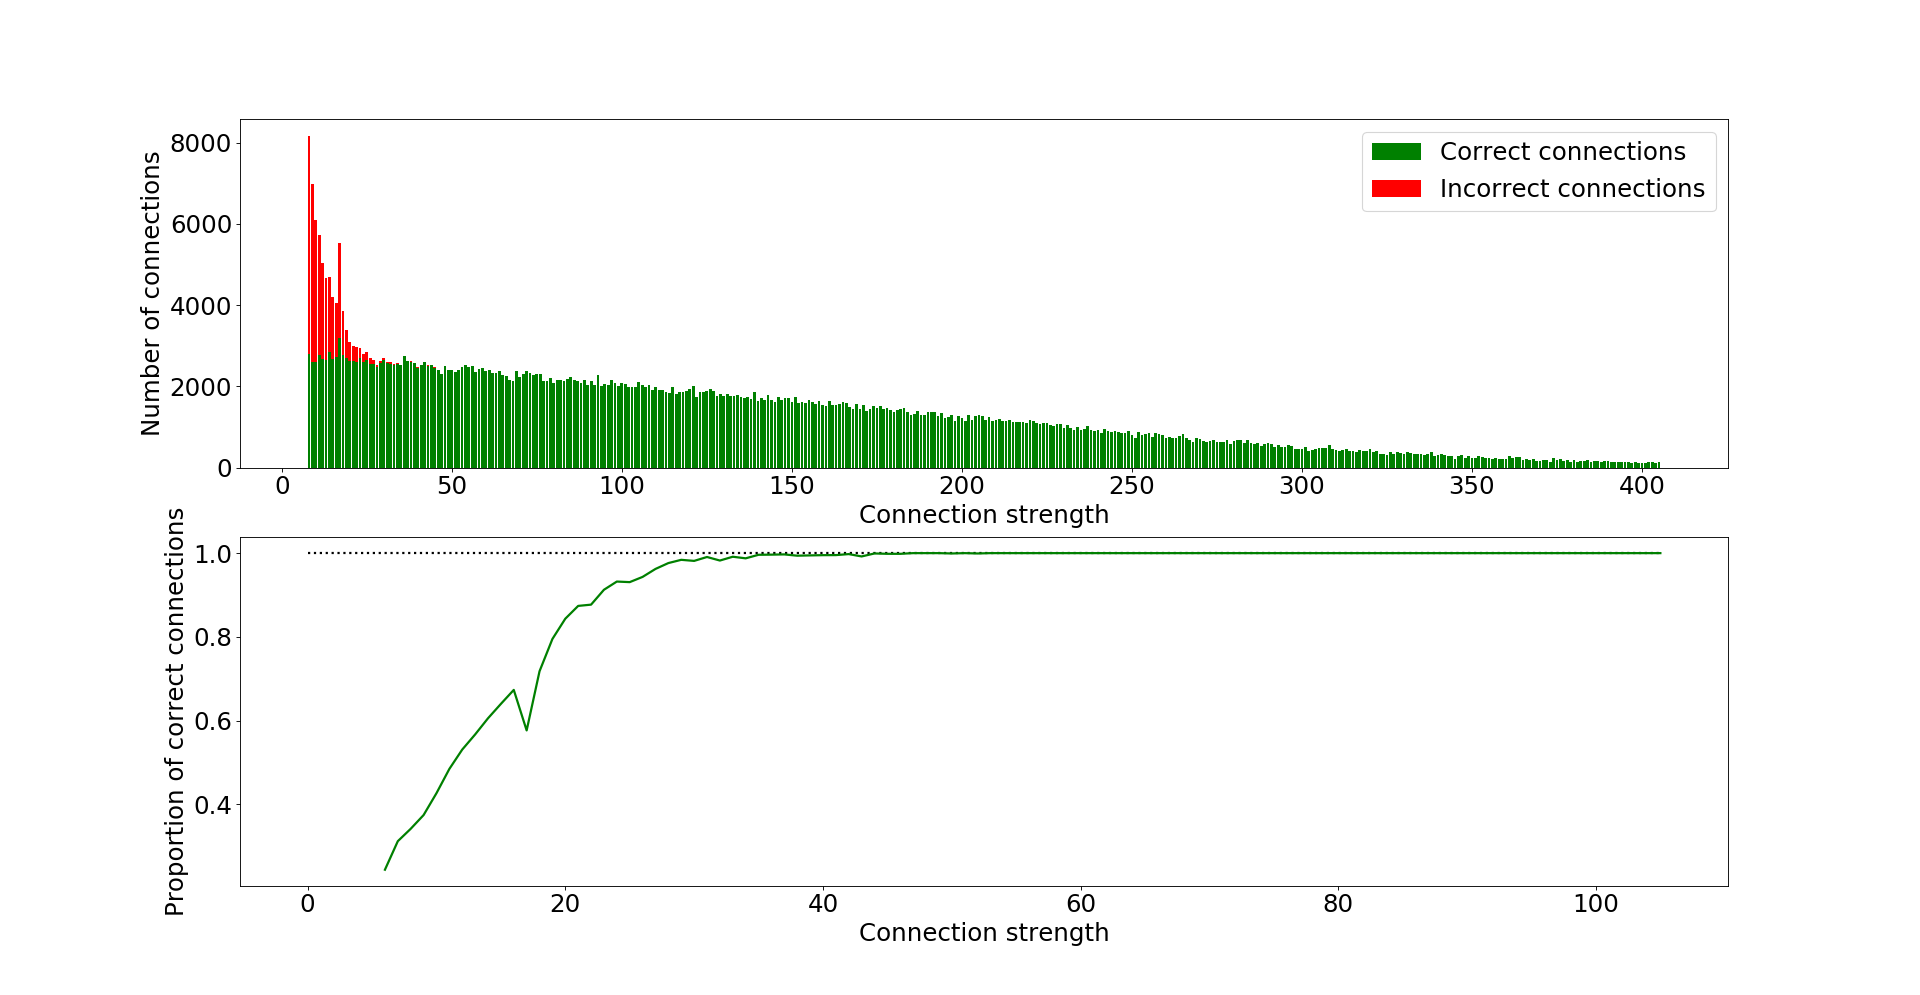
\includegraphics[width=400bp]{figures/artificial_conn.png}
\caption{On top, histogram of connections in RNP50 color coded by their correctness. On bottom, the relation between number of shared SDKs and a proportion of correct connections.}
\label{fig:artificial_conn}
\end{figure}

For demonstration purposes, we ran spectral clustering (a combination of embedding and clustering) on the RIL50 dataset ($\approx$6400 reads) with SDK set chosen as described in the previous chapter. More specifically, we use Self-Tuning Spectral Clustering\cite{zelnik2005self} embedding into a 10-dimensional space. In order not to overload the graph with a lot of spurious edges that connect unrelated reads, we only considered the connections with strength at least 5. A histogram of these connections can be observed on figure \ref{fig:artificial_conn}.

To construct an entry in the similarity matrix for reads $r_1$ and $r_2$, we rescale the strength of the connection $(r_1, r_2)$ to a range $\left[ 0.3, 20\right]$ and exponentiate it. This is done as to accentuate the differenced between weakly and strongly connected reads.

$$A[r_1, r_2] = e^{rescale(strength(r_1, r_2))}$$

The results are encouraging : the combination of spectral embedding and clustering yields seven 100\% pure components with evenly distributed sizes containing almost all of the reads.

However, applying the same pipeline to a more realistic dataset, such as that of E.coli strains is not feasible due to computational complexity. Calculating the eigenvectors of an $N \times N$ matrix takes in general $O(N^3)$ time, but even if that could be reduced, the $O(N^2)$ memory required for the graph Laplacian matrix is enough of a disqualifying factor for datasets of hundreds of thousands of reads.

If we are to use a method such as spectral embedding, a drastic reduction in the number of treated objects is necessary. As such, we first apply a different heuristic resulting in high-purity components the quantity of which is several orders of magnitude lower.

\section{Forming scaffold components}

\begin{figure}
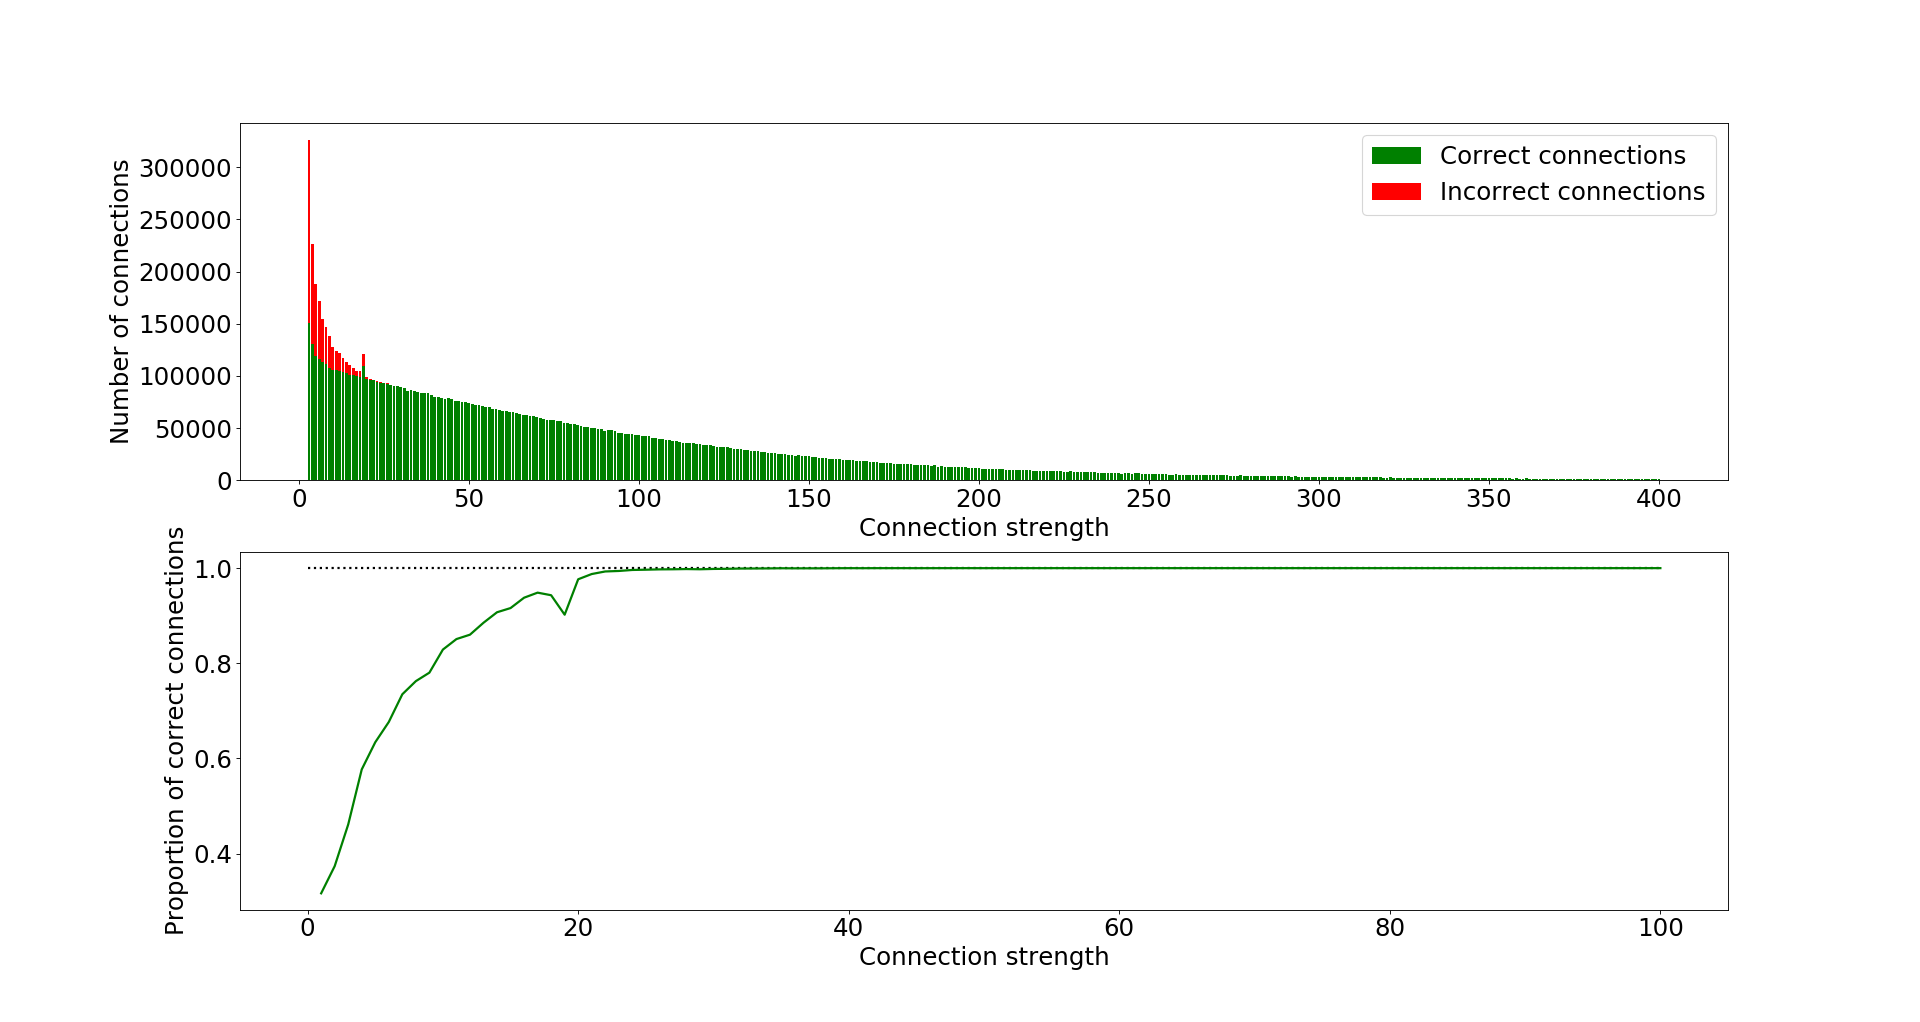
\includegraphics[width=400bp]{figures/connections_initial.png}
\caption{Same type of histogram as \ref{fig:artificial_conn}, but for ENP75}
\label{fig:conn_init}
\end{figure}

If we take a closer look at the figure \ref{fig:conn_init}, we can see that beyond a certain threshold value for the number of shared SDKs, all of the implied edges in our graph are correct.

The exact value of this threshold seems to depend on a few factors, such as:
\begin{itemize}
	\item{The length distribution of the reads - shorter reads contain less SDKs, so the threshold is also lower}
	\item{Error profile of the used sequencing platform - errors eliminate SDKs from the reads, lowering the threshold}
	\item{Fraction of $k$-mers in SDK set that are not true DK - higher contamination rate implies higher threshold}
	\item{Abundance of SDKs - the higher percentage of reads in $k$-mers are SDKs, the higher the threshold, since along with true DK we also grow the set of contaminant SDKs}
\end{itemize}

In all of our experiments with ENP75 and EPB75 datasets, this validity threshold however never exceeded 70 shared $k$-mers and there is little reason to suspect that the value should be dramatically higher for real datasets - after all, the purpose of the simulation software is to model the first two points of the above list as closely to reality as possible.

Knowing there is a safe threshold, we can guess its upper bound, or rather what percentage of all edges sorted by their strengths in descending order we can consider to be “correct”. We set our guess to be the top 15\% of all the edges (for ENP75 and EPB75 datasets the actual safe threshold would be met even with top ~50\% of edges).

Assuming that all of our guessed edges are correct, we can use these to connect their respective vertices into components and expect these components to be 100\% pure at the end. The fastest way to realize these connections is using a union-find algorithm, with the edges sorted by their weights in descending order on the input.

On the output of our union-find we receive a list of formed components, along with a spanning tree of edges used to form them. We call the components created by this first round of union-find scaffold components.

At this point, it is important to realize just what the strong connections represent: reads that share a high number of suspected discriminative $k$-mers not only come from the same haplotype, but they also cover intersecting intervals of bases in the haplotype genome.

\begin{figure}
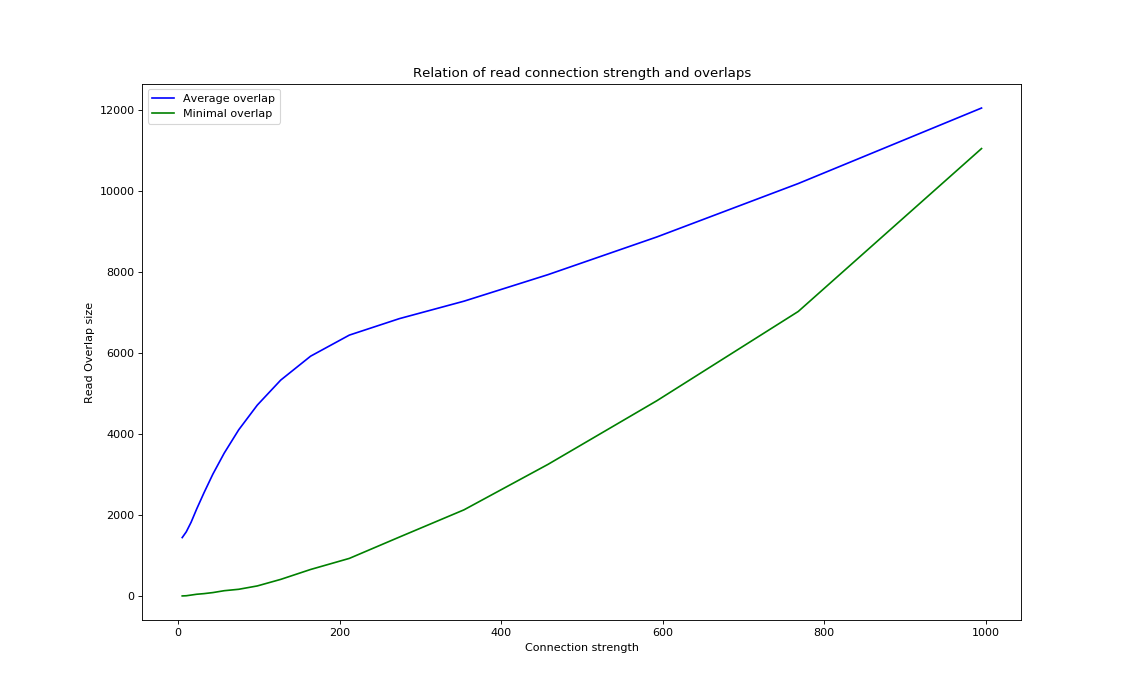
\includegraphics[width=400bp]{figures/overlap_relation.png}
\caption{Relation between number of shared SDKs between reads and the size of their overlap (as determined by read metadata)}
\label{fig:overlap_relation}
\end{figure}

Therefore, by finding strong connections between reads we in a way also find local alignments between reads. It closely follows that by performing union-find on a set of reads we are also creating a spanning tree of read alignments.

Moreover, for adjacent reads in the spanning tree that have overlapping intervals (which in the case of our trees are all the adjacencies), we can construct a larger interval by overlapping them. By induction, it would follow that every path in the tree corresponds to one interval in the haplotype genome.

We visualize one such tree on figure \ref{fig:tree} using a force-directed layout, where vertices repel each other but are held together by edges.

\begin{figure}
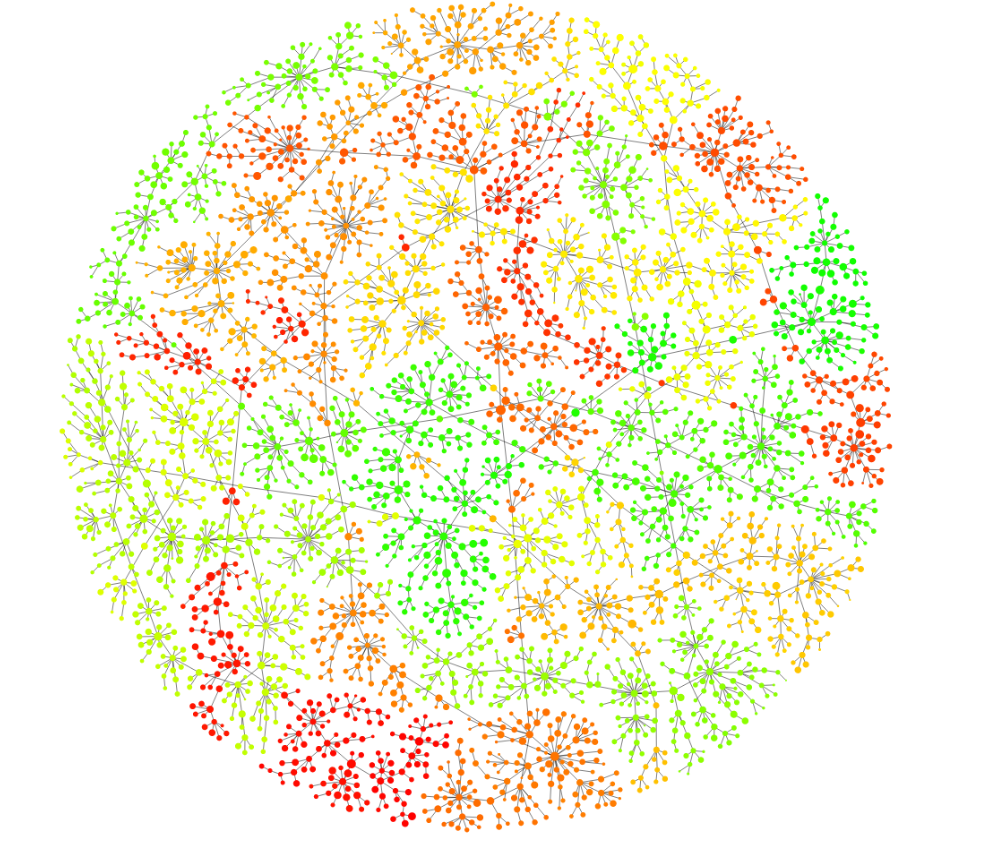
\includegraphics[width=450bp]{figures/tree.png}
\caption{Scaffold component rendered using its spanning tree, with edges connecting reads}
\label{fig:tree}
\end{figure}

The vertices in figure \ref{fig:tree} are color coded according to the value of the middle of their interval. The larger the value, the farther right the vertex is on a green-to-red spectrum, and the  larger the dot, the longer the visualized reads are. As can be seen, the only instances when the two neighboring vertices have a noticeably different color happen between pairs, where at least one vertex is relatively big. This can be expected, as in case of Nanopore reads, the read lengths often exceed tens of thousands of bases.

For the ENP75 dataset the described union-find step with connection strength threshold manually set to the lowest possible safe value (51 shared SDKs) managed to create two scaffold components containing reads, the intervals of which covered the vast majority of their respective haplotypes. 

With our conservatively chosen 15\% of top connections however, the number of found scaffold components rises, but not dramatically - at worst we obtained a couple dozen components. We expect to get no more than a few hundred components even for very large datasets with larger than bacteria genomes. Note that our union-find procedure connects together only a fraction of all the reads in our dataset - in the case of ENP75, it was about two thirds of all reads. We will deal with the remaininder at a later point.

\section{Component intervals}

Let us define a function $overlap\_intervals$ operating on the interval data provided by simulated reads:

\begin{figure}[H]
\lstset{language=Python}
\begin{lstlisting}[basicstyle=\small]
type Position = int
type IsStart = bool
Interval = namedtuple(start=int, end=int)

def overlap_intervals(intervals: List[Interval]) -> List[Interval]:
    interval_endpoints: List[Tuple[Position, IsStart]]
    for interval in intervals:
        interval_endpoints.append((read.start, True))
        interval_endpoints.append((read.start, False))
    interval_endpoints.sort()

    overlapped_intervals = []
    opened_start = -1
    opened_intervals_count = 0
    for position, is_start in interval_endpoints:
        if is_start:
            opened_intervals_count += 1
            if opened_intervals_count == 1:
                opened_start = position
        else:
            opened_intervals_count -= 1
            if opened_intervals_count == 0:
                overlapped_intervals.append(Interval(opened_start, position))
    return overlapped_intervals

\end{lstlisting}
\caption{Method that overlaps intervals, forming larger interval(s)}
\label{fig:overlap_method}
\end{figure}

Function $overlap\_intervals$ creates the largest intervals it can by overlapping the intervals of reads contained within a component.

Let us use the function Intervals on the calculated scaffold components of ENP75. The output for each haplotypes components can be seen in tables \ref{table:comp_intervals_a} and \ref{table:comp_intervals_b} and is sorted by the start of the interval(s).

\begin{table}[]
	\begin{tabular}{|l|l|l|l|}
	\hline
	\textbf{Component size} & \textbf{Interval start} & \textbf{Interval end} & \textbf{Overlap with next} \\ \hline
	4204                    & 462832                  & 1154974               & 11380                      \\ \hline
	10295                   & 1143594                 & 2736534               & 11691                      \\ \hline
	3736                    & 2724843                 & 3341829               & 4680                       \\ \hline
	495                     & 3337149                 & 3452186               & 6647                       \\ \hline
	3050                    & 3445539                 & 3945210               & 15198                      \\ \hline
	1531                    & 3930012                 & 4181787               & 19827                      \\ \hline
	1060                    & 4161960                 & 4357072               & 9031                       \\ \hline
	4867                    & 4348041                 & 465672                & 2840                       \\ \hline
	\end{tabular}
\caption{Component sizes, intervals, and interval overlaps for MG1655 reads}
\label{table:comp_intervals_a}
\end{table}

\begin{table}[]
	\begin{tabular}{|l|l|l|l|}
	\hline
	\textbf{Component size} & \textbf{Interval start} & \textbf{Interval end} & \textbf{Overlap with next} \\ \hline
	141                     & 194306                  & 235740                & 12817                      \\ \hline
	1676                    & 222923                  & 471448                & 10355                      \\ \hline
	4766                    & 461093                  & 1204808               & 12363                      \\ \hline
	3799                    & 1192445                 & 1781958               & 9452                       \\ \hline
	297                     & 1772506                 & 1837607               & 10216                      \\ \hline
	6415                    & 1827391                 & 2794482               & 9736                       \\ \hline
	506                     & 2784746                 & 2882149               & 13047                      \\ \hline
	4605                    & 2869102                 & 3562204               & 3918                       \\ \hline
	461                     & 3558286                 & 3648611               & 13086                      \\ \hline
	58                      & 3635525                 & 3666623               & 6569                       \\ \hline
	273                     & 3660054                 & 3731855               & 11106                      \\ \hline
	3045                    & 3720749                 & 4207882               & 7347                       \\ \hline
	741                     & 4200535                 & 4327655               & 8092                       \\ \hline
	6487                    & 4319563                 & 200444                & 6138                       \\ \hline
	\end{tabular}
\caption{Component sizes, intervals, and interval overlaps for UTI89 reads}
\label{table:comp_intervals_b}
\end{table}
\textit{Note : the intervals wrap around because E.coli has a circular genome}

As we can see, for each component, only one interval was created. This is understandable, since all the adjacent reads in the component overlap with their intervals. 
What is crucial however, is that the intervals between scaffold components of the same category overlap as well. Interestingly, they only seem to overlap by the tails of their intervals : this can be explained by a following thought experiment:

The overlapping tails $T_1$ and $T_2$ of intervals correspond to two sets of reads $R_1$ and $R_2$ that share a (potentially empty) set of SDKs $S$. Suppose we grow the overlap, and therefore both the tails, along with the sets $R_1, R_2$ and as a consequence grow the set $S$. The more we grow the set $S$ however, the more likely it is that there exists a read $R_{common}$ which is sufficiently long and with sufficiently many SDKs contained in $S$ that would bridge the two tails during the union-find phase, contradicting the creation of these tails in the first place. Therefore, the only overlaps we find are relatively short - in our case, their length is only a few average read lengths high.

From the above findings it follows that if we had a way of locating the overlaps, we could merge the scaffold components into even larger components, potentially ending up with only one very large component per each haplotype. Moreover, it can be seen that if we were to construct an interval by using these overlaps, the result would cover the entirety of the haplotype sequence.

At this point it would be tempting to use the same method of calculating connections through shared SDKs as before, but this time between the scaffold components. This however does not work : as can be seen, the component intervals only overlap by a small percentage of their lengths. This means that only the shared SDKs between reads that constitute these overlapping “tails” of components can be trusted to create a correct connection. Since we do not know which these reads are within a component, we would need to consider all the SDKs of a component when calculating a connection. This however results in the contaminating SDKs often outweighing the “trustworthy” SDKs, causing the strongest connections to be incorrect.

\section{Connecting scaffold components}

\subsection{Longest path in a spanning tree}

Recall the analogy of a path in the spanning tree of the scaffold component that represents one interval in the haplotype. If we could find the path representing the longest interval, we would also find the reads that form the aforementioned tails of said interval. On real data, we of course do not know the interval for any read - we only have an approximation (due to insertions and deletions) of its length. We also do now know how long the overlaps between the connected reads are. This however, we can approximate using the SDKs.

Let us define a function $estimate\_overlap$ operating on a pair of reads. We assume a pre-computed nested hash-map $kmer\_positions$ containing the positions of SDKs within reads is available.

\begin{figure}[H]
\lstset{language=Python}
\begin{lstlisting}[basicstyle=\small]
def estimate_overlap(Read x, Read y) -> int:
    shared_kmers = intersection(x.discriminative, y.discriminative)

    x_positions, y_positions = [], []
    for kmer in shared_kmers:
        x_positions.append(kmer_positions[x][kmer])
        y_positions.append(kmer_positions[y][kmer])

    max_x = max(x_positions)
    min_y = min(x_positions)
    max_y = max(y_positions)
    min_y = min(y_positions)

    return max(max_x - min_y, max_y - min_y)
\end{lstlisting}
\caption{Method for calculating approximate overlap between reads}
\label{fig:estimate_overlap}
\end{figure}

Function $estimate\_overlap$ calculates for a pair of reads the approximate length of their overlap based on the positions of $k$-mers that the two reads share. Assuming that most $k$-mers in the SDK set are really discriminative, this approximation will in an overwhelming proportion of cases undervalue the true length of overlap, as can be seen on figure \ref{fig:overlap_error} depicting the distribution of error for ENP75. This undervaluation however, is not significant (less than half a percent in most cases).

\begin{figure}
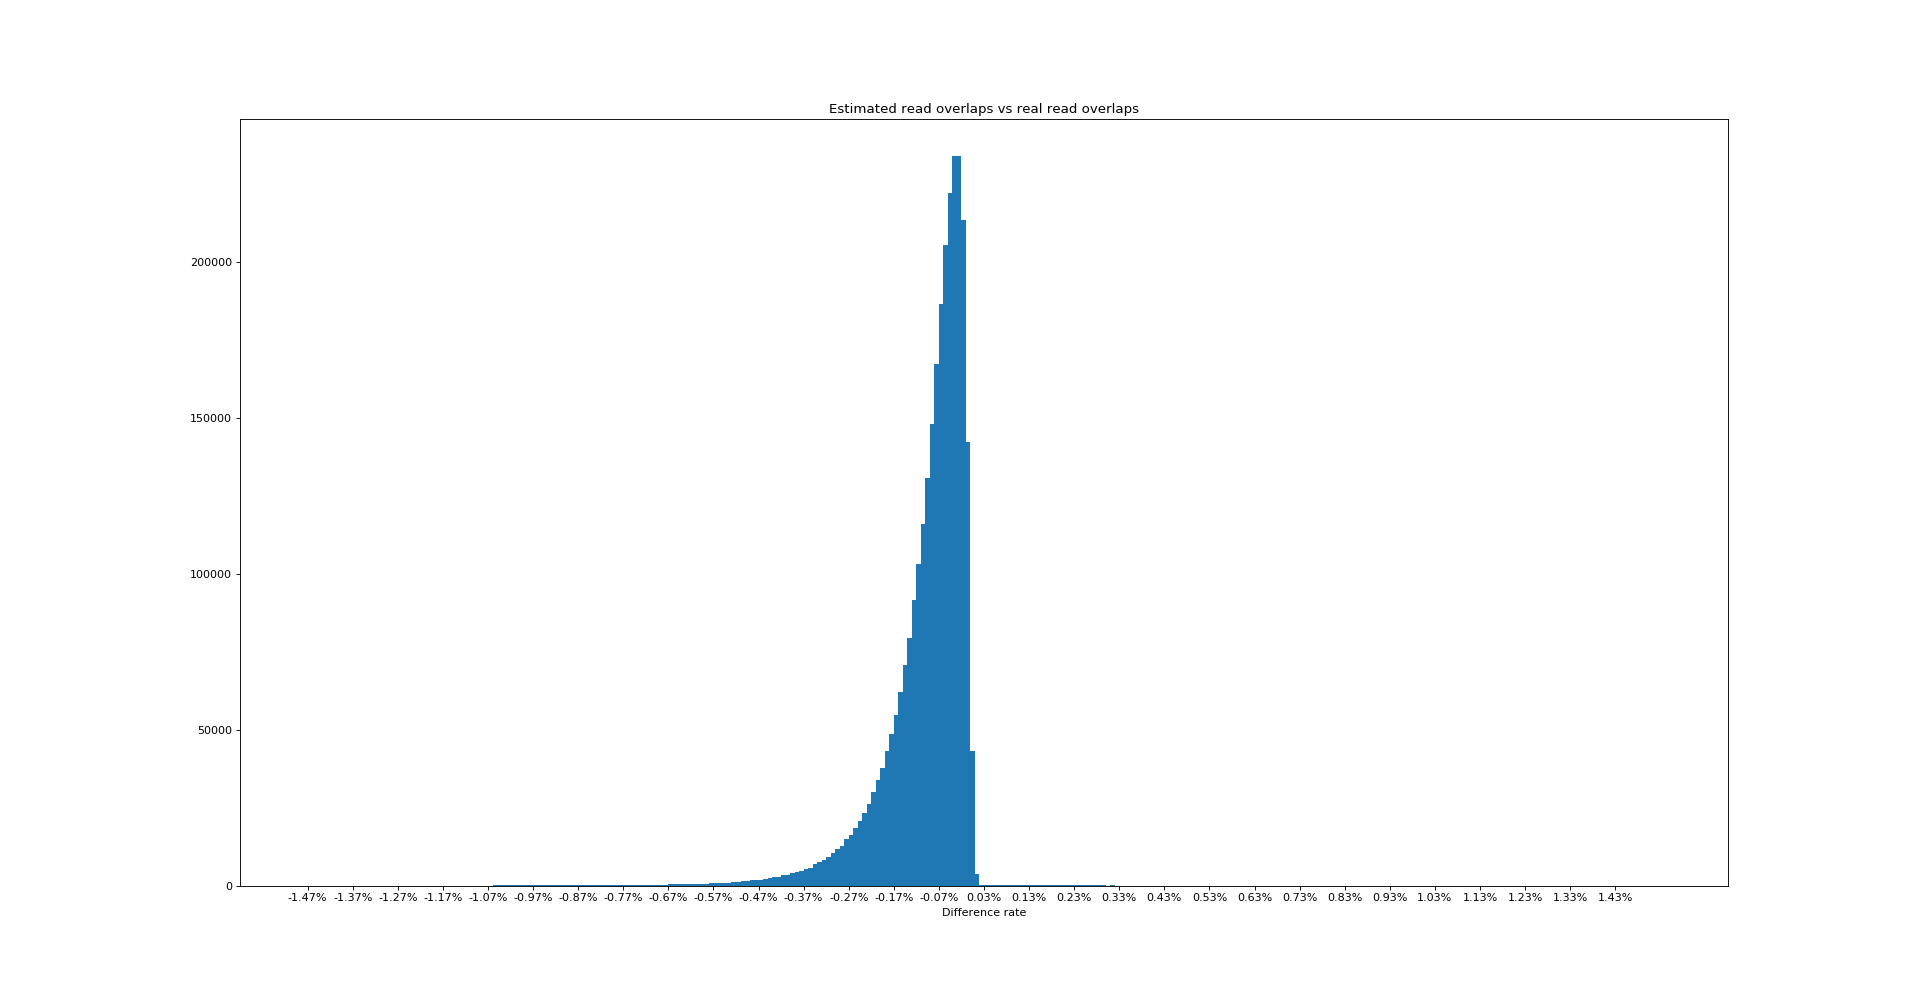
\includegraphics[width=400bp]{figures/overlap_error.png}
\caption{Error distribution of calculated overlap lengths vs. real overlap lengths}
\label{fig:overlap_error}
\end{figure}

Knowing the approximate overlap size between reads along with their lengths, we define a length metric on the spanning tree of reads as follows:

Let $P = (v_1, v_2, ... v_k)$ be a path in the spanning tree of reads. Let $read\_length(v_i)$ be a function outputting the length of a read represented by vertex $v_i$. We define a length function on paths to be:

$$path\_length(P) = \sum_{i = 1}^{k}{read\_length(v_i)} - \sum_{i = 1}^{k - 1}{estimate\_overlap(v_i, v_{i + 1})}$$

We are using the length function $path\_length$ as a substitute for the unavailable read intervals. As will become apparent later, the approximation provided by this function is quite accurate.

Now that we have a length metric for the paths in the spanning tree which is usable for real data, we can proceed with finding the longest path, and eventually the vertices on the tails.
Fortunately, finding a longest path in an acyclic undirected graph such as ours is relatively easy. We will use an adaptation of an algorithm ordinarily used for finding the diameter of a tree\cite{diameter}. Let us define a function $distance\_bfs$ operating on an adjacency list constructed from a spanning tree.

\begin{figure}[H]
\lstset{language=Python}
\begin{lstlisting}[basicstyle=\small]
type Vertex = int
type Distance = int

def distance_bfs(start: Vertex, adjacency: dict):
    vertex_queue = Queue()
    vertex_queue.push(starting)
    visited = set()
    dist = {start: read_length[start]}

    while (!vertex_queue.empty()):
        c = vertex_queue.pop()
        visited.add(c)
        if c not in adjacency:
            continue

        for n, distance in adjacency[c].items():
            if n in visited:
                continue
            dist[n] = dist[c] + read_length[n] - estimate_overlap(n, c)
            vertex_queue.push(n)

    return distances

\end{lstlisting}
\caption{Method for calculating distances from one vertex in the spanning tree to all the other}
\label{fig:distance_bfs}
\end{figure}

Function $distance\_bfs$ calculates distances from a starting vertex to all other vertices using the length function $path\_length$ as distance-increasing metric.

In the first run we start from an arbitrary vertex $v_{start}$ of our tree $T$. We find a vertex $v_{farthest}$ that is the most distant from $v_{start}$. It can be proved by contradiction that $v_{farthest}$ is one of the boundary vertices on the longest path.

Starting from $v_{farthest}$, we run $distance\_bfs$ again, obtaining a map of distances $D_{left}$. Again, we query the vertex from $D_{left}$ with the maximum distance. We will call this vertex $v_{left}$.

Finally, we run $distance\_bfs$ a third time from $v_{left}$, obtaining a map of distances $D_{right}$. The vertex with maximum distance in this map is the same one as $v_{farthest}$. We relabel it as $v_{right}$. 

The path that can be traced from $v_{left}$ to $v_{right}$ is the longest path in the tree $T$.
In the first three columns of table \ref{table:tail_intervals} we can observe how closely related are intervals for the found boundary reads $v_{left}$, $v_{right}$ with the overarching interval of the entire tree (scaffold component). For convenience, we occasionally swapped values of $v_{left}$ and $v_{right}$, as their order is not important for our calculations.

\begin{table}[]
\begin{tabular}{|l|l|l|l|l|}
\hline
\textbf{$v_{left}$ start} & \textbf{$v_{right}$ end} & \textbf{component int.} & \textbf{$Tail_{left}$ start} & \textbf{$Tail_{right}$ end} \\ \hline
469260                 & 1154083               & 462832-1154974          & 462832                   & 1154974                 \\ \hline
4172298                & 4352140               & 4161960-4357072         & 4161960                  & 4357072                 \\ \hline
3453190                & 3945210               & 3445539-3945210         & 3445539                  & 3945210                 \\ \hline
3349388                & 3452186               & 3337149-\textbf{3452186}         & \textbf{3339053}         & 3452186                 \\ \hline
2725664                & 3341829               & 2724843-3341829         & 2724843                  & 3341829                 \\ \hline
3930012                & 4176215               & 3930012-4181787         & 3930012                  & 4181787                 \\ \hline
1144647                & 2731271               & 1143594-2736534         & 1143594                  & 2736534                 \\ \hline
\end{tabular}
\caption{Intervals of scaffold components compared to computed boundary read and tails intervals}
\label{table:tail_intervals}
\end{table}

We can see that while not perfectly accurate, the boundary reads $v_{left}, v_{right}$ cover intervals the ends of which are very close to the actual ends of the interval for the whole component. The inaccuracy is caused by the estimative nature of both read lengths and overlaps.

We can however do better. If one recalls, the point of our interest are reads that constitute the tails of the component interval - and we do not necessarily have to only take the two edge-most ones. Instead of only taking the two reads $v_{left}, v_{right}$ that are the farthest apart, we can instead take a set of reads $Tail_{left}, Tail_{right}$, where $Tail_{left}$ is a set that is “sufficiently distant” from $v_{right}$ and $Tail_{right}$ is a set “sufficiently distant” from $v_{left}$.

In our case, we define “sufficiently distant” as being no more than two average read lengths less distant, than the most distant vertex. This variable is set as such based on the observed overlap length between scaffold component intervals from tables \ref{table:comp_intervals_a} and \ref{table:comp_intervals_b} which does not seem to depend on the overall interval length.

As can be seen per last three columns of table \ref{table:tail_intervals}, the bounds of intervals for tails strike the component interval bounds dead on with only one exception. 
To give a visual clue as to which vertices are included in the tail sets, we present figure \ref{fig:tails}, an altered version of figure \ref{fig:tree}. In the figure, the left tail vertices are highlighted in green, while the right tail vertices are red.

\begin{figure}
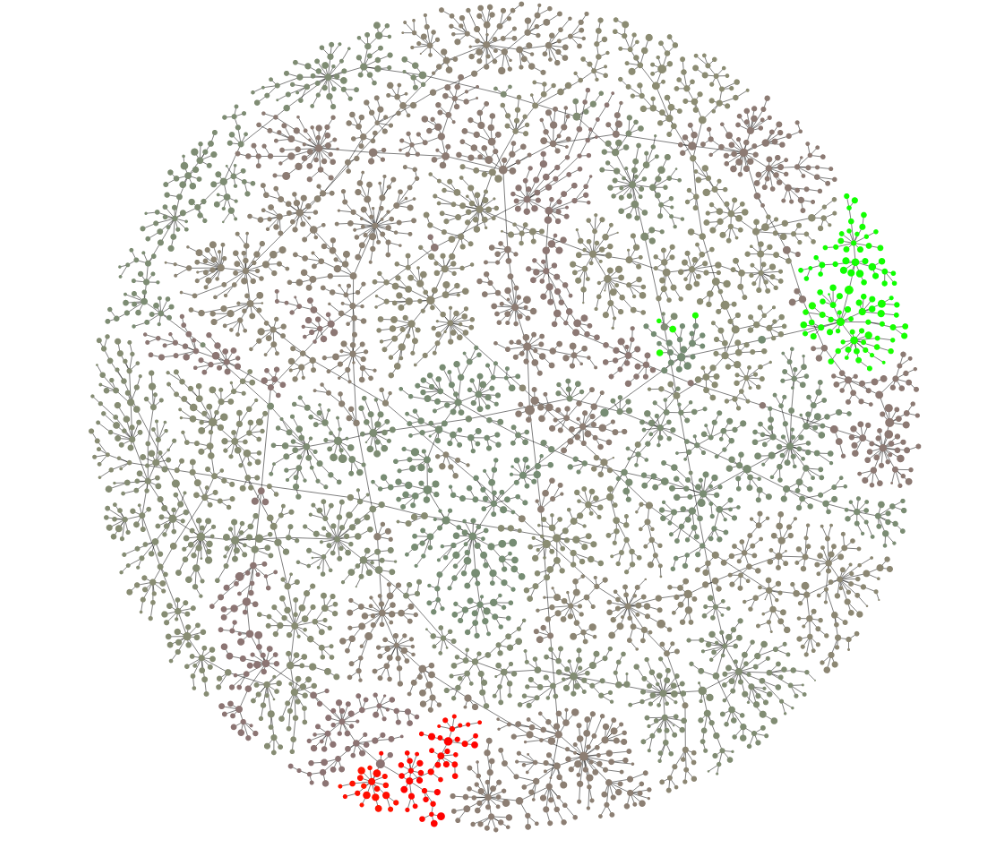
\includegraphics[width=450bp]{figures/tails.png}
\caption{Highlighted sets of vertices $Tail_{left}$ and $Tail_{right}$}
\label{fig:tails}
\end{figure}

Now that we have located the tail reads/vertices of our component spanning trees, we can proceed with calulating connections between them. It's only logical that we again use the number of shared SDKs as the metric, but this time the SDKs for a tail are an aggregate of the SDKs for the reads contained within said tails.
In order to ensure our tails contain as many SDKs from the tail interval as possible, we perform an additional step of their “amplification”. The idea is, that since we have many reads that went unused during the formation of scaffold components, we can link some of these to our tails to ensure we capture as many SDKs belonging to the tails intervals as possible. As we will see later, vertices that we temporarily “borrow” this way will end up in the same component eventually.

As such, during amplification we calculate connections from the tail vertices into the set of unused vertices, and incorporate the SDKs of strongly connected (a set constant for number of shared SDKs) into the set of SDKs for the tail. 

\begin{figure}[H]
\lstset{language=Python}
\begin{lstlisting}[basicstyle=\small]
def amplified_tail_SDKs(tail: List[Vertex]) -> Set[Kmer]:
    amplified_tail = tail[::]
    for connection in get_connections(from=tail, minimal_score=40):
        amplified_tail.append(connection.to)

    amplified_tail_SDKs = {}
    for vertex in amplified_tail:
        amplified_tail_SDKs.add(vertex.discriminative_kmers)

    return amplified_tail_SDKs
\end{lstlisting}
\caption{Method for amplifying a tail of a spanning tree}
\label{fig:amplification}
\end{figure}

We can now proceed with calculation of connections between scaffold components. For each pair of components $C_1$ and $C_2$, we compute the number of shared SDKs between the:
\begin{itemize}
	\item{Right tail of $C_1$ and right tail of $C_2$}
	\item{Right tail of $C_1$ and left tail of $C_2$}
	\item{Left tail of $C_1$ and right tail of $C_2$}
	\item{Left tail of $C_1$ and left tail of $C_2$}
\end{itemize}
We take only the maximum of the four computed values and set it to be the connection strength between $C_1$ and $C_2$.

For the ENP75 dataset which yielded 22 scaffold components in the union-find step, we end up with 151 cross-tail connections with strength higher than zero. A graph of this size is small enough to reintroduce spectral clustering as a viable clustering method.

Using Self-Tuning spectral clustering\cite{clustering_lib}, we managed to reduce the number of components down to 4, with two components per each haplotype.

\begin{figure}
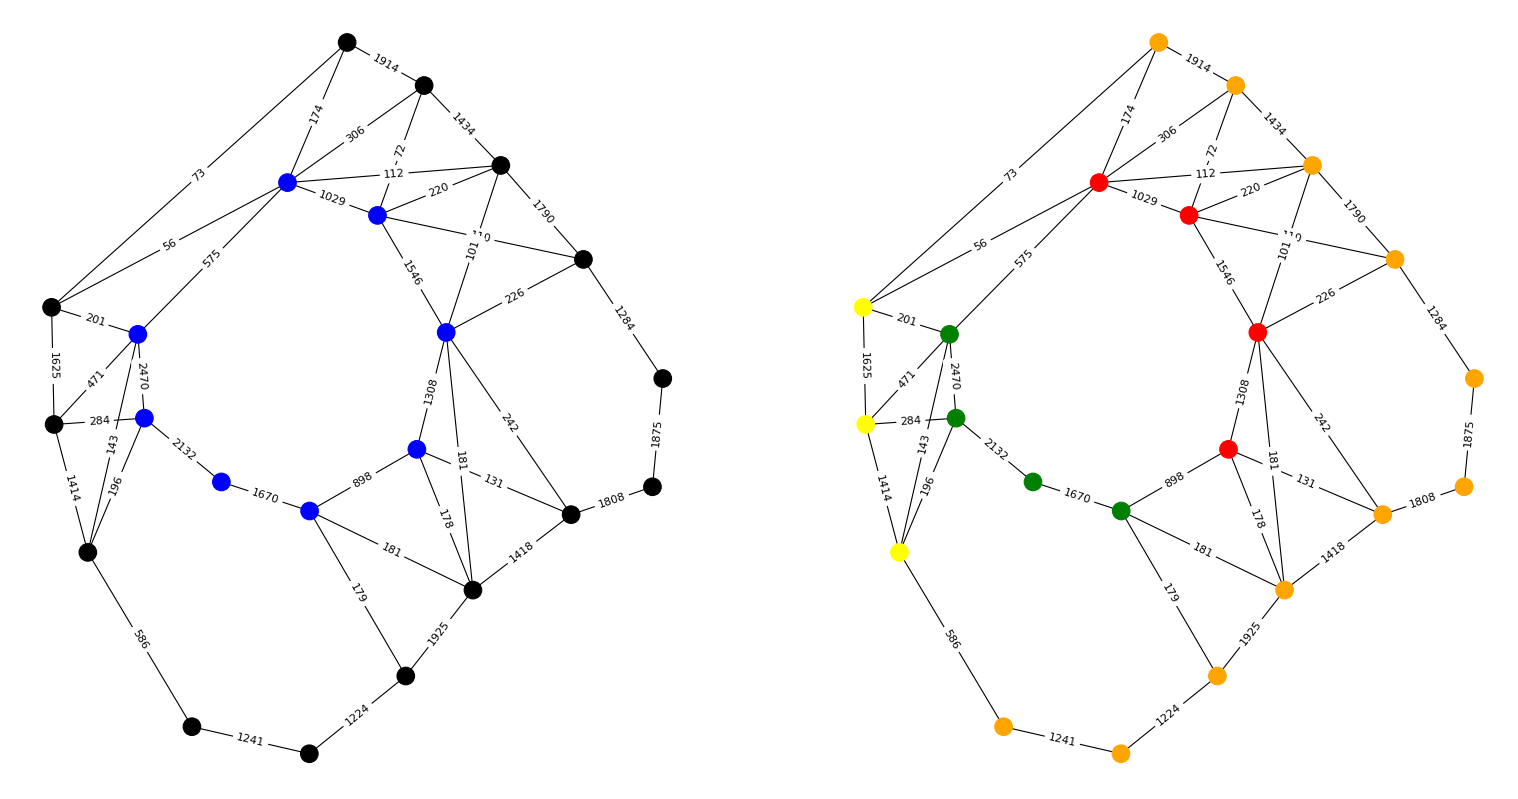
\includegraphics[width=450bp]{figures/spectral2.png}
\caption{Graph of scaffold components and tail connections between them. Correct categorization on the left, clusters found by spectral clustering on the right. Edges with strengths lower than 50 not displayed for brevity}
\label{fig:tails}
\end{figure}

We call the components on the output of spectral clustering Core components. From this point on, we will not merge any two Core components together.

\section{Enrichment of core components}

Now that we have core components which are few in number and together likely span the entirety of all haplotypes, we can direct our focus on resolving the status of all the reads that were left out during the formation of scaffold components. 

The process of enrichment is similar to the union-find step we already used, except this time, we calculate only the connections between core components and the unresolved reads, and the union-find is restricted from ever joining together core components. Thanks to this fact, upon calculation of connections we can already tell to which core component a read is going to be assigned, allowing us to plot a figure of realized connections, as shown on figure \ref{fig:conn_enrich}.

\begin{figure}
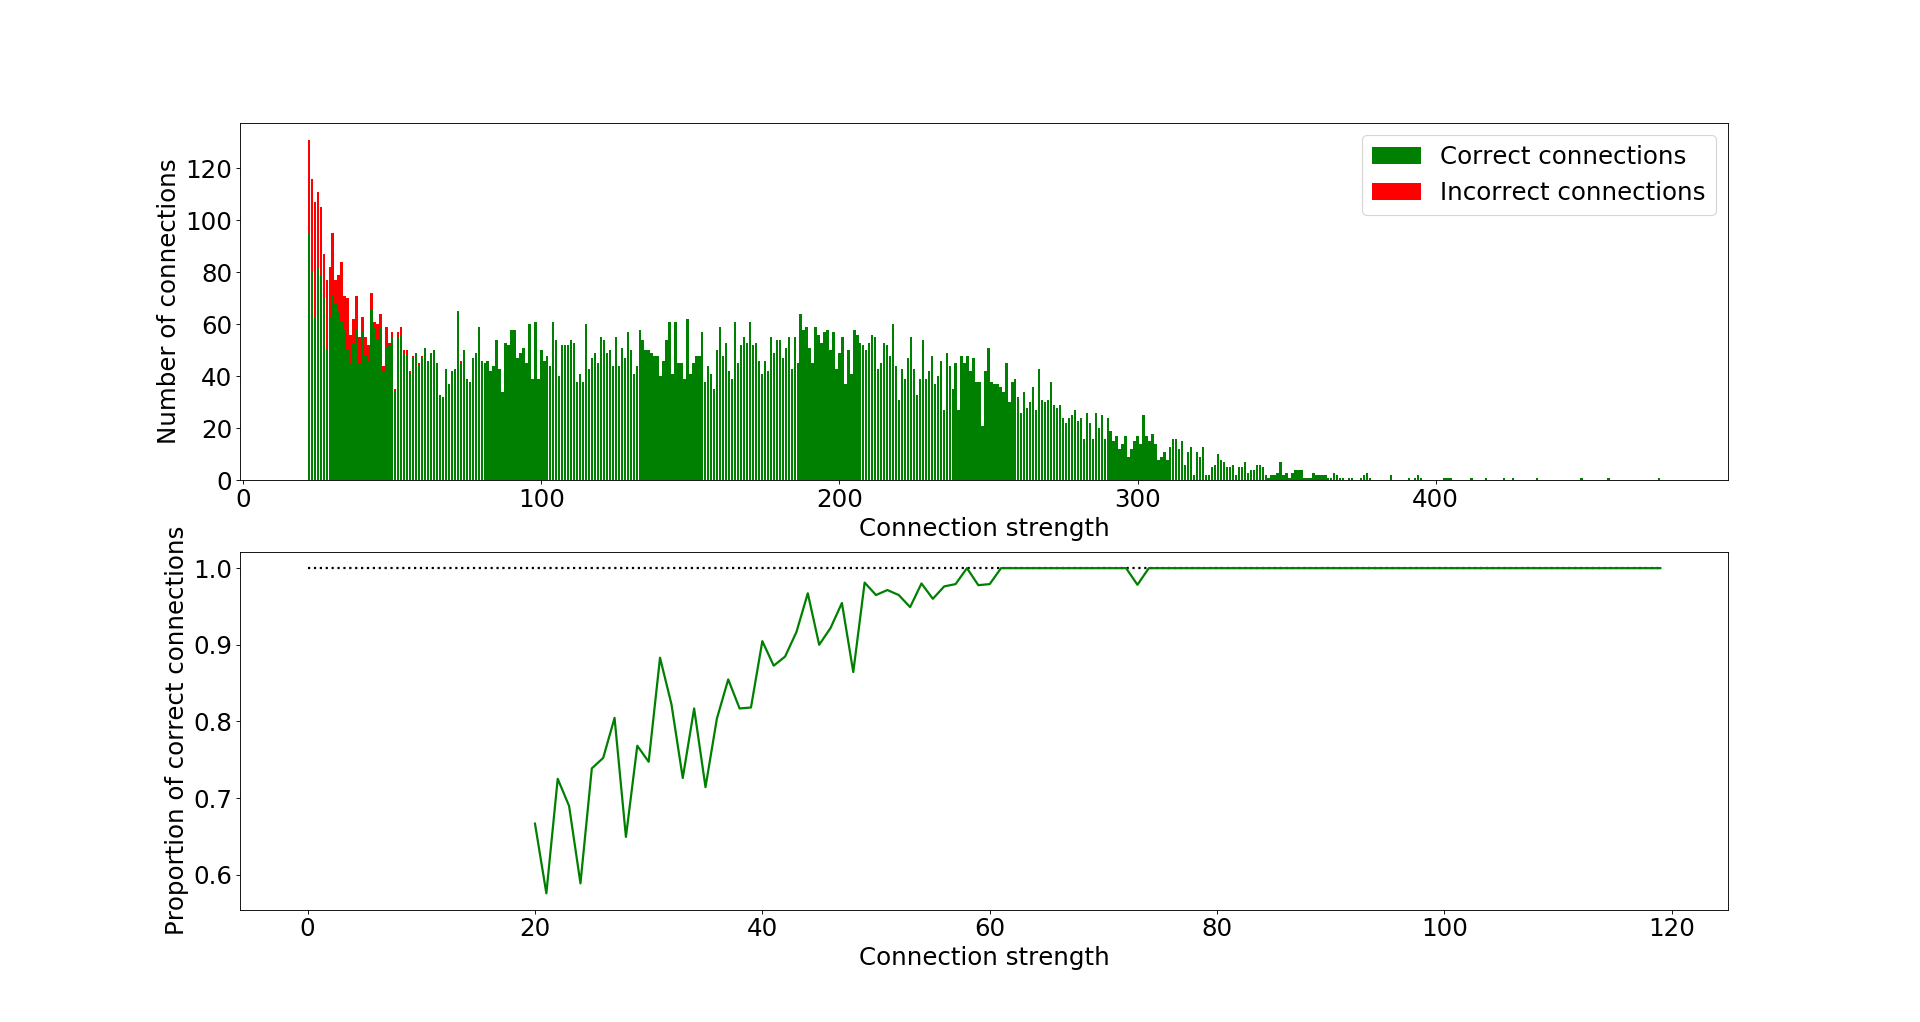
\includegraphics[width=400bp]{figures/connections_enrichment.png}
\caption{On top, histogram of connections in ENP75 color coded by their correctness. On bottom, the relation between number of shared SDKs and a proportion of correct connections.}
\label{fig:conn_enrich}
\end{figure}

The practical effect is that most unresolved reads are assigned to the core component to which they have the strongest connection. Again, we set a limit to the minimal strength of a connection to be used during the union find. We found that for the E.coli dataset, going to as low as 20 shared SDKs is viable without introducing more than one percent of impurity to our core components.

\begin{figure}
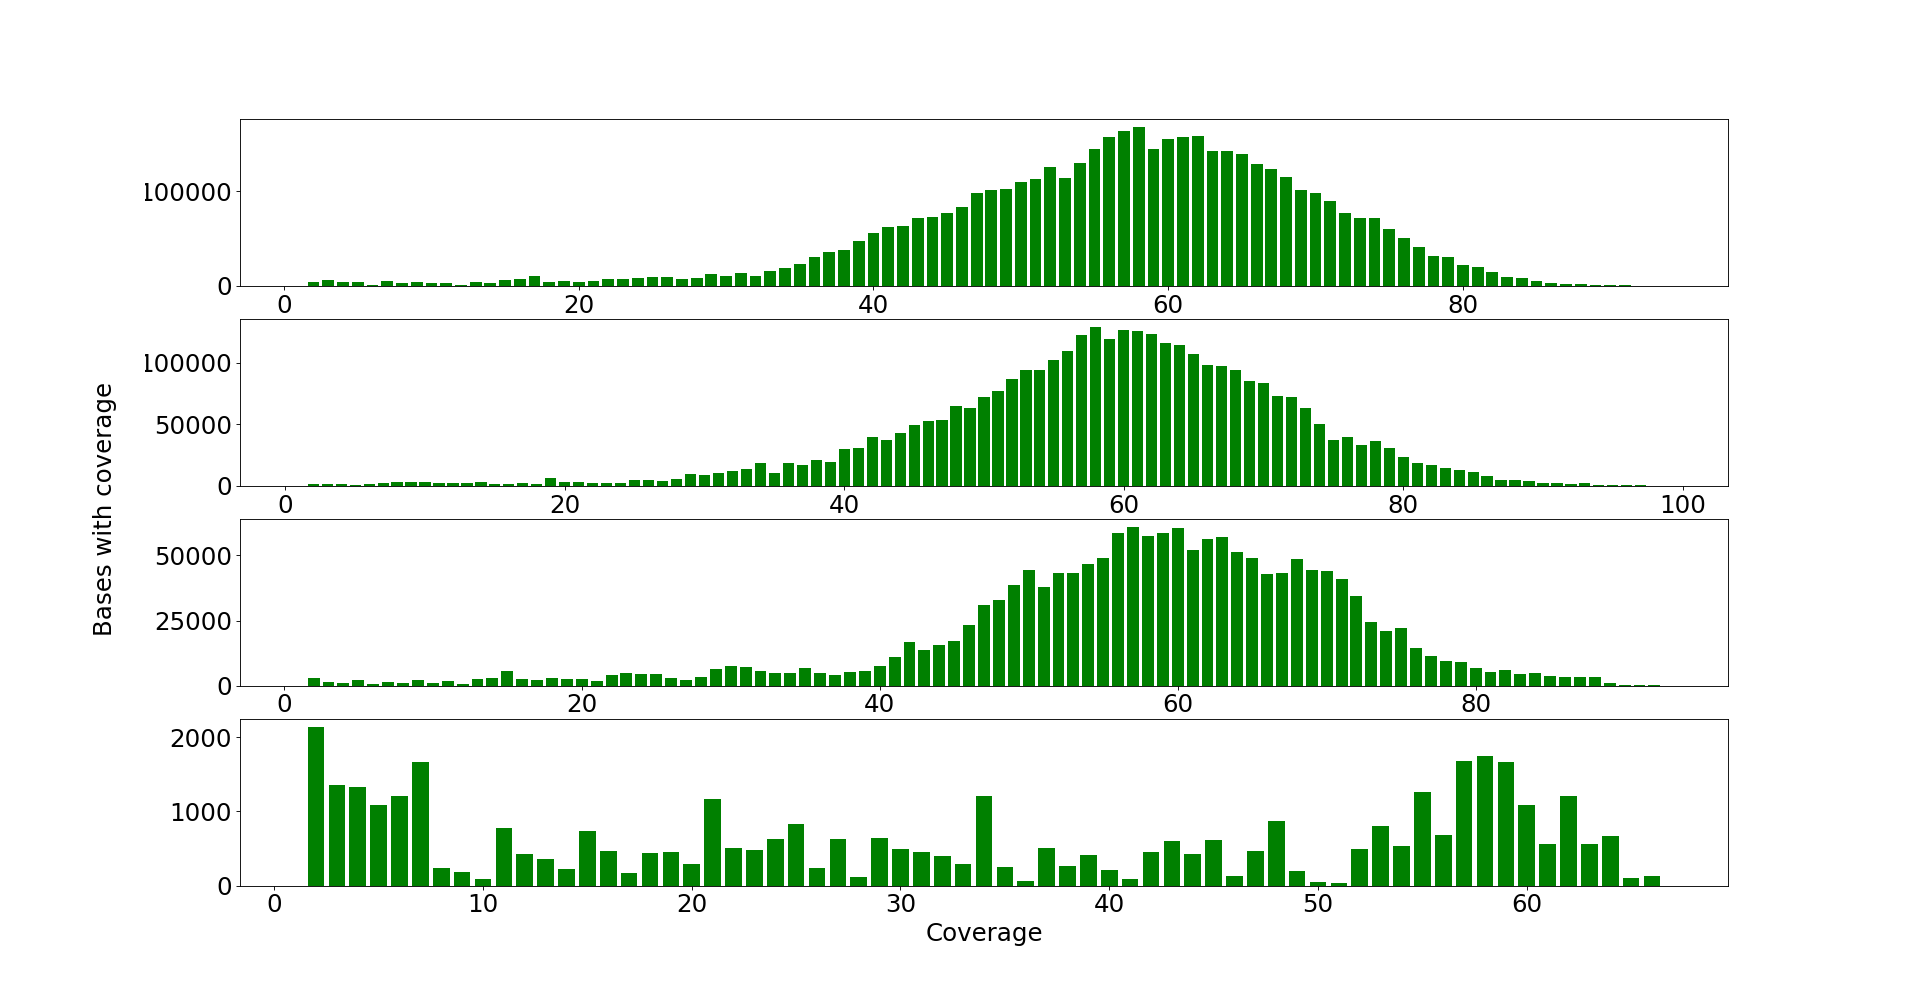
\includegraphics[width=450bp]{figures/coverage_before.png}
\caption{Histogram of coverage within components before enrichment}
\label{fig:coverage}
\end{figure}

\begin{figure}
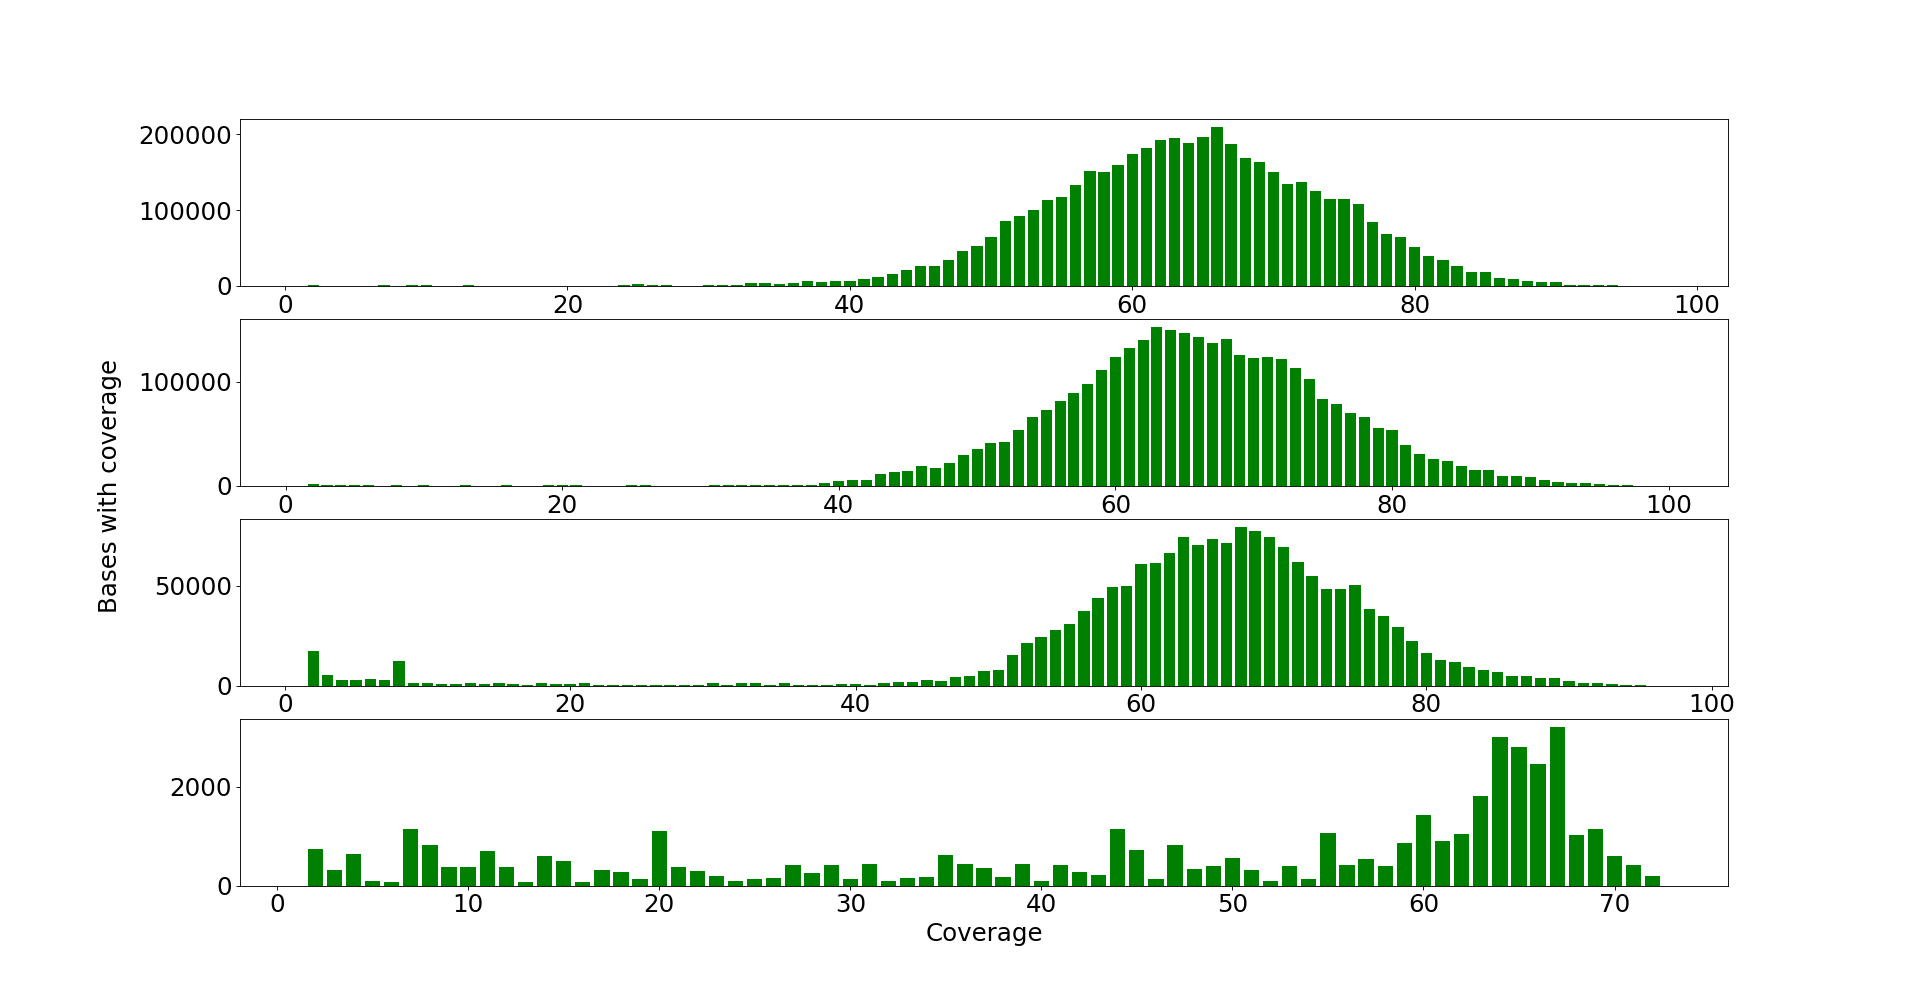
\includegraphics[width=450bp]{figures/coverage_enriched.png}
\caption{Histogram of coverage within components after enrichment. We can see that enrichment visibly improved the overal coverage in the last component}
\label{fig:coverage_enriched}
\end{figure}

The difference in coverage caused by enrichment is depicted on figures \ref{fig:coverage} and figure \ref{fig:coverage_enriched}.

The enriched components constitute the final result of our algorithm.